% Options for packages loaded elsewhere
\PassOptionsToPackage{unicode}{hyperref}
\PassOptionsToPackage{hyphens}{url}
%
\documentclass[
  landscape]{article}
\usepackage{lmodern}
\usepackage{amssymb,amsmath}
\usepackage{ifxetex,ifluatex}
\ifnum 0\ifxetex 1\fi\ifluatex 1\fi=0 % if pdftex
  \usepackage[T1]{fontenc}
  \usepackage[utf8]{inputenc}
  \usepackage{textcomp} % provide euro and other symbols
\else % if luatex or xetex
  \usepackage{unicode-math}
  \defaultfontfeatures{Scale=MatchLowercase}
  \defaultfontfeatures[\rmfamily]{Ligatures=TeX,Scale=1}
\fi
% Use upquote if available, for straight quotes in verbatim environments
\IfFileExists{upquote.sty}{\usepackage{upquote}}{}
\IfFileExists{microtype.sty}{% use microtype if available
  \usepackage[]{microtype}
  \UseMicrotypeSet[protrusion]{basicmath} % disable protrusion for tt fonts
}{}
\makeatletter
\@ifundefined{KOMAClassName}{% if non-KOMA class
  \IfFileExists{parskip.sty}{%
    \usepackage{parskip}
  }{% else
    \setlength{\parindent}{0pt}
    \setlength{\parskip}{6pt plus 2pt minus 1pt}}
}{% if KOMA class
  \KOMAoptions{parskip=half}}
\makeatother
\usepackage{xcolor}
\IfFileExists{xurl.sty}{\usepackage{xurl}}{} % add URL line breaks if available
\IfFileExists{bookmark.sty}{\usepackage{bookmark}}{\usepackage{hyperref}}
\hypersetup{
  pdftitle={Caso BOPS},
  pdfauthor={Jorge Salvador Ruiz Montaño},
  hidelinks,
  pdfcreator={LaTeX via pandoc}}
\urlstyle{same} % disable monospaced font for URLs
\usepackage[margin = 1.1cm]{geometry}
\usepackage{graphicx,grffile}
\makeatletter
\def\maxwidth{\ifdim\Gin@nat@width>\linewidth\linewidth\else\Gin@nat@width\fi}
\def\maxheight{\ifdim\Gin@nat@height>\textheight\textheight\else\Gin@nat@height\fi}
\makeatother
% Scale images if necessary, so that they will not overflow the page
% margins by default, and it is still possible to overwrite the defaults
% using explicit options in \includegraphics[width, height, ...]{}
\setkeys{Gin}{width=\maxwidth,height=\maxheight,keepaspectratio}
% Set default figure placement to htbp
\makeatletter
\def\fps@figure{htbp}
\makeatother
\setlength{\emergencystretch}{3em} % prevent overfull lines
\providecommand{\tightlist}{%
  \setlength{\itemsep}{0pt}\setlength{\parskip}{0pt}}
\setcounter{secnumdepth}{-\maxdimen} % remove section numbering
\usepackage{booktabs}
\usepackage{longtable}
\usepackage{array}
\usepackage{multirow}
\usepackage{wrapfig}
\usepackage{float}
\usepackage{colortbl}
\usepackage{pdflscape}
\usepackage{tabu}
\usepackage{threeparttable}
\usepackage{threeparttablex}
\usepackage[normalem]{ulem}
\usepackage{makecell}
\usepackage{xcolor}

\title{Caso BOPS}
\author{Jorge Salvador Ruiz Montaño}
\date{23/11/2020}

\begin{document}
\maketitle

\hypertarget{secciuxf3n-c}{%
\subsection{Sección C}\label{secciuxf3n-c}}

\hypertarget{c.1-bops}{%
\subsubsection{C.1 BOPS}\label{c.1-bops}}

Resuelve el caso \textbf{Evaluating BOPS at Home and Kitchen}

\begin{enumerate}
\def\labelenumi{\arabic{enumi}.}
\item
  ¿Deberían expandirse a Canadá?
\item
  ¿Cuántos millones de dólares se ganaron o perdieron a partir del
  programa? Explica tu razonamiento y metodología.
\end{enumerate}

\begin{itemize}
\tightlist
\item
  Como nos dice el caso, se realizó un estudio tomando como base las DMA
  (Designed Market Areas) que son las áreas donde se concentra el mayor
  número de posibles clientes dentro de un radio definido.
\item
  Ahora tenemos dos tipos de mediciones, antes de antes de lanzar BOPS y
  otras después de lanzar BOPS.
\item
  Usando estos datos podemos comparar como fluctuó la venta por DMA y
  además podemos separar aquellos DMA que estabán cerca de una tienda y
  lejos de una tienda (Radio de 50 millas), lo cual puede influir
  bastante en el uso de BOPS ya que se requiere que el cliente recoja su
  producto en tienda.
\item
  Se realizaron 3 graficas para comparar la venta online a nivel DMA en
  (USA) y por BM en Cánada, se tomaron en cuenta todas la suma de la
  venta de todas las tiendas por semana.
\end{itemize}

\newpage

\hypertarget{resultados-de-dmas-cercanas.}{%
\subsubsection{Resultados de DMAs
cercanas.}\label{resultados-de-dmas-cercanas.}}

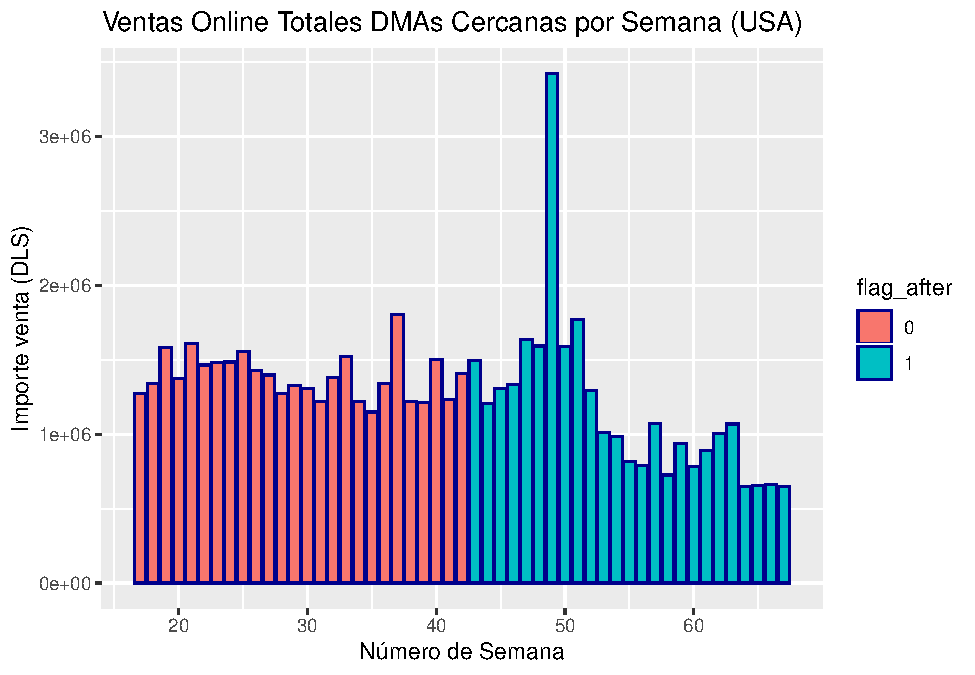
\includegraphics{R_BOPS_files/figure-latex/exportando_datos_DMAs_Cerca-1.pdf}

\begin{itemize}
\tightlist
\item
  Se puede observar como la venta online tendió a bajar después de que
  se lanzó BOPS (exceptuando el pico por ventas de fin de año).
\end{itemize}

\hypertarget{resultados-de-dmas-lejanas.}{%
\subsubsection{Resultados de DMAs
lejanas.}\label{resultados-de-dmas-lejanas.}}

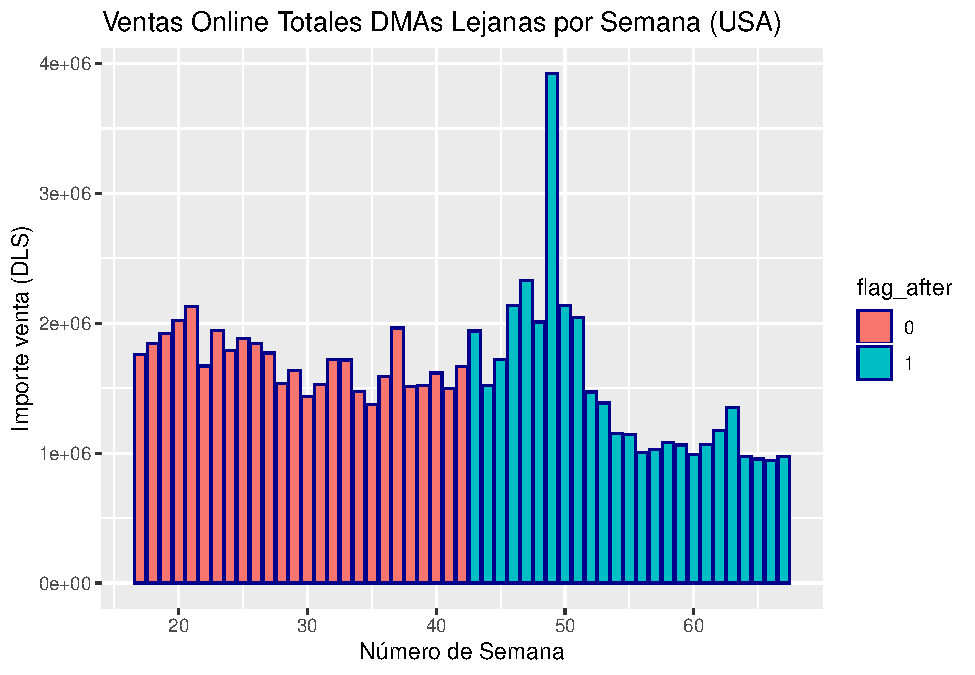
\includegraphics{R_BOPS_files/figure-latex/DMAs_Lejanas-1.pdf}

\begin{itemize}
\tightlist
\item
  cabría esperar que las ventas de tiendas lejanas tuviera una
  distribución diferente a las cercanas, pero demos ver casi la misma
  tendencia, lo que nos dice que a los usuarios no les importa mucho el
  lugar donde se encuentra la tienda física al comprar en Linea.
\end{itemize}

\hypertarget{resultados-de-venta-bm-en-canaduxe1}{%
\subsubsection{Resultados de Venta BM en
Canadá}\label{resultados-de-venta-bm-en-canaduxe1}}

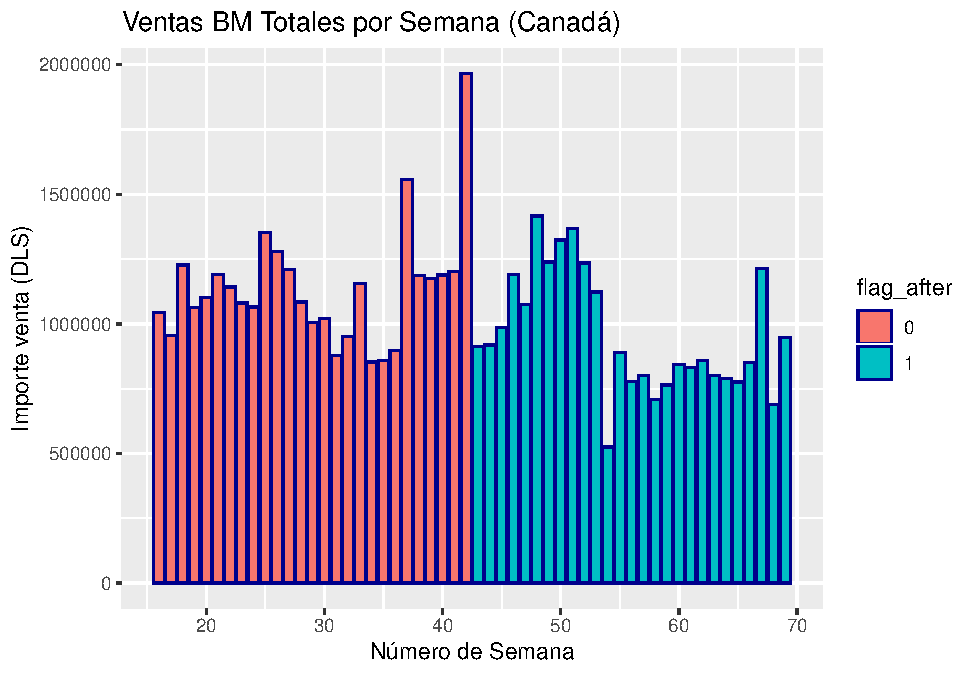
\includegraphics{R_BOPS_files/figure-latex/venta_BM_canada-1.pdf}

\begin{itemize}
\tightlist
\item
  La ventas en Cánada por BM también están bajando luego de incorporar
  BOPS en USA, puede ser débido a los problemas de lógista que arrastra
  la empresa debido a BOPS.
\end{itemize}

\hypertarget{conclusiones}{%
\subsubsection{Conclusiones}\label{conclusiones}}

\begin{itemize}
\item
  Dado que la tendencia en las ventas online no se ve afectada por el
  sitió de la tienda física, a los clientes no se les ve muy motivados a
  usar BOPS y recoger sus productos en tienda. Al menos en USA. Mi
  recomendación sería no expandir BOPS a Canadá si no se tiene cambios
  en la tendencia de venta online que favorezcan a las tiendas que se
  encuentran cerca del cliente. Se podrían trazar indicadores como de \%
  de compra por BOPS vs envios a domicilio por DMA.
\item
  En cuanto a lo que se perdió debido a DMAs, viene en la descripción
  del problema (a grandes razgos) que fueron \$2000 DLS en promedio por
  DMA y \$7545 DLS en promedio por tienda física, por tiempo no será
  posible hacer una estimación más a fondo de las pérdidas, pero se
  podría hacer sacando totales de las ventas antes y después (mismas que
  use para las gráficas) de BOPS o utilizando el promedio de pérdidas y
  el total de BOPS y tiendas registradas.
\end{itemize}

\end{document}
